\documentclass[11pt, a4paper]{article}
\usepackage[T2A]{fontenc}
\usepackage[utf8]{inputenc}
\usepackage[bulgarian]{babel}

%% Sets page size and margins
\usepackage[a4paper,top=3cm,bottom=3cm,left=3cm,right=3cm,marginparwidth=1.75cm]{geometry}

%% Useful packages
\usepackage{amsmath, amssymb, amsthm,calc,mathabx}
\usepackage{systeme}
\usepackage{graphicx}
\usepackage[colorinlistoftodos]{todonotes}
\usepackage[colorlinks=true, allcolors=black]{hyperref}
\usepackage{wrapfig,lipsum,booktabs}
\usepackage{enumitem}
\usepackage{float}
\usepackage{fmtcount}
\usepackage{multicol}
\usepackage{breqn}
\usepackage{setspace}
\usepackage{hyperref}
\usepackage{mathtools}
\usepackage {tikz}
\usetikzlibrary {positioning}
\usetikzlibrary{shapes.geometric}
\graphicspath{
	{Graphics/}
	{Graphics/BackupFunction/}
}
\newtheorem{theorem}{Theorem}

\newtheorem{lemma}{Lemma}
\newtheorem{prop}{Property}
\newtheorem*{remark}{Remark}

\theoremstyle{definition}
\newtheorem{definition}{Дефиниция}

\setlength{\columnsep}{1cm}
\setlength{\parindent}{1em}

\newcommand\blfootnote[1]{%
	\begingroup
	\renewcommand\thefootnote{}\footnote{#1}%
	\addtocounter{footnote}{-1}%
	\endgroup
}

\begin{document}
\begin{titlepage}
	\newcommand{\HRule}{\rule{\linewidth}{0.5mm}}
	\centering
	\textsc{\LARGE УК БАН '19}\\
	
\includegraphics[width=0.5\textwidth]{Uchimi_logo}\\
	\HRule\\[1 cm]
	{\huge\bfseries Рансъмуер и Устойчиви Стратегии за Архивиране}\\[1 cm]
	\HRule\\
	\vfill
			\Large
			\textit{Автор:}
			 \textsc{Никола Стайков}\\
             \vspace{2cm}
			\Large
			\textit{Ментор:}
            \textsc{Явор Папазов}
    \vfill	
	{\large\today}   
	\vfill
\end{titlepage}

\tableofcontents
\newpage
\begin{abstract}
		Рансъмуер е вид компютърен вирус, който критптира файловете на дадена система и изисква да бъде платен откуп, за да бъдат декриптирани. Създателите на рансъмуер могат да правят малки проучвания преди да започнат основната кампания с цел да определят гореспоменатото разпределение. Първата част на този проект разглежда модел, чрез който да бъдат определени оптималните параметри за едно такова проучване. Главната и най-ефективна защита срещу рансъмуер е правенето на архиви. Те на свой ред обаче могат да представляват съществен разход за големите компании, поради което трябва да бъдат внимателно планирани. Това е взето предвид във втората част на проекта, в която е разгледан модел за архивиране на данни, състоящ се от пълни и инкрементални архиви, и е изчислена очакваната цена за възстановяване на данните. Процесът по възстановяване е пресъздаден и анализиран чрез визуализация на python и Монте Карло симулация.
\end{abstract}

\section{Въведение}
		Този проект е разделен на две основни части, разглеждащи съответно модели за оптимизиране на откуп и оптимизиране на архивиране. Изследвайки обстойно двете противоположни позиции, можем да създадем пълна представа за стратегиите едновременно на атакуващите и жертвите. Обмисляйки начини как всяка от двете страни може да подобри стратегията си ни дава идея как да направим стабилна защитна стратегия чрез архивиране.
\section{Теория}
	В тази част са включени всички дефиниции и концепции, които са нужни за цялостното разбиране на проекта.
		\begin{definition}
			\label{def:normdist}
			\emph{Нормално разпределение}, означено  с $N(\mu, \sigma)$, е вид непрекъснато разпределение, където с $\mu$, $\sigma$ и $\sigma^{2}$ са означени среднoто аритметично, стандартната девиация и вариацията съответно.
		\end{definition}
	
		Графиката на тази функция образува крива, често наричана също камбанна крива. Тя има максимум $(x,f(x))$ в $\left(\mu, \dfrac{1}{\sigma\sqrt{2\pi}}\right)$:
		\begin{center}
			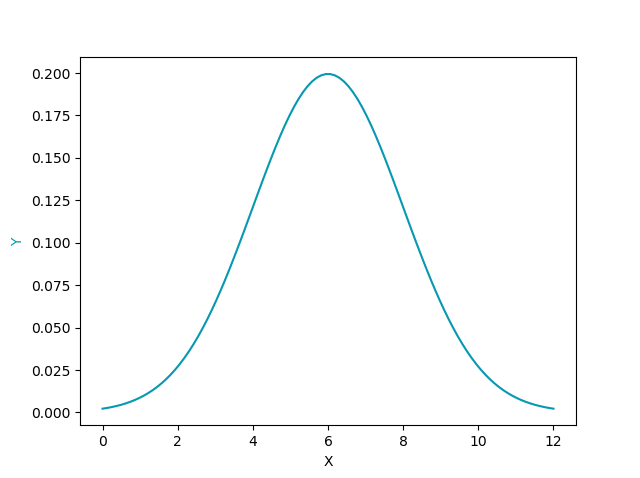
\includegraphics[width=0.6\textwidth]{Normal_clean}
		\end{center}
		
		\begin{definition}
			\label{def:def2}
			Разглеждаме нормално разпределение $N(\mu, \sigma)$. \emph{Стандартната стойност}, или \emph{Z-score}, на дадено $x$ показва колко стандартни девиации е то от дадената средна стойност. Пресмята се по формулата $\dfrac{x-\mu}{\sigma}$.
		\end{definition}
	
		\begin{definition}
			\label{def:prob_dist}
			За дадено разпределение \emph{функцията на разпределение} $F(x)$ показва вероятността стохастична променлива, следваща разпределението, да е по-малка или равна на $x$
			$$F_{X}(x)=\mathbb{P}(x\leq X).$$
		\end{definition}
	
		\begin{definition}
			\label{def:prob_dens}
			\emph{Плътност на разпределение} на непрекъсната стохастична променлива $x$, описва вероятността дадена стохастична променлива $x$ да се окаже в произволен интервал. Формално се дефинира чрез
			\begin{align*}
				&\mathbb{P}(x < X \leq x+\Delta)=F_X(x+\Delta)-F_X(x)\\
				&f_X(x)=\lim_{\Delta \rightarrow 0} \frac{F_X(x+\Delta)-F_X(x)}{\Delta}.		
			\end{align*}
		\end{definition}
	
		\begin{definition}
			\label{def:err}
			\emph{Грешка от първи род} е резултат на интегрирането на нормално разпределение, тя приема z-score като параметър и пресмята интеграла между фиксирана точка и средната стойност за разпределението.
			$$\operatorname{erf}(z)=\dfrac{2}{\sqrt{\pi}}\int_{0}^{z}e^{-t^{2}}dt.$$
		\end{definition}
	
		\begin{definition}
			\label{def:Bernoulli_trial}
			\emph{Опит на Бернули} е стохастичен експеримент с два изхода и фиксирани вероятности за провал и успех:
			\begin{center}
				$P(\text{успех})=p$\\
				$P(\text{провал})=1-p.$
			\end{center}
		\end{definition}
		
		\begin{definition}
			\label{def:Binomial_distribution}
			\emph{Биномно разпределение} е статистическото разпределение на изходите (успех/провал) при провеждането на определен брой опити на Бернули.
			За $n$ опита и вероятност за успех $p$ вероятността точно $k$ от тях да са успешни е:
			$$
			P(\text{успех} = k) = \frac{\binom{n}{k}p^{k}(1-p)^{n-k}}{2^k}
			$$
		\end{definition}
		\newpage

	\section{Оптимизиране на откуп}		
		\subsection{Въведение}
			Рансъмуер се появява за първи път през 1989 под формата на the AIDS Troyan, познат също като PC Cyborg.  The AIDS Trojan е бил доста лесен за преодоляване, тъй като използва симетрична криптография, и скоро са били разработени начини файловете да бъдат декриптирани, но този случай поставя началото на развитието на много от модерните заплахи. С навлизането на Интернет, рансъмуер се завръща с нова сили, а именно с the Archiveus Trojan и GPcode от 2006. Друг повратен момент в историята на рансъмуер е създаването на биткойн, и крипто-валутите като цяло, по много причини, някои от тях бидейки анонимността и автоматичните и невъзвръщаеми транзакции\cite{huang2018tracking}.\par
			В изминалите години е имало опити да бъде направен модел на пазара на malware. В \cite{caulfielddynamic}, авторите са създали теоретичен модел, взимайки предвид броя потребители, които имат архиви, както и други фактори като разпространението на информация и надеждност на рансъмуер.           
			В \cite{cartwright2018pay} е изследван различен подход, който разглежда възможността за допълнително уговаряне на цената като игра между жертвата и престъпниците. Тази разработка се фокусира на теория на игрите и комбинаторика.\par
			Доста усилия са положени и за проследяването на плащания, свързани с рансъмуер в блокчейн, тъй като всички те са публични. В резултат на това има публични данни, свързани с тези плащания, предоставени от \cite{paquet2019ransomware} и в \cite{thomas2015framing} човек може да се запознае с много заключенияв, подкрепени с данни, отнасящи се не само до рансъмуер, но и до целия черен пазар.\par
			Моделът в настоящата разработка е базиран на описания в \cite{caulfielddynamic}, но се фокусира върху оптимизирането на параметри, които не са разгледани в споменатата статия.
		\subsection{Подход}
			Този модел описва разпространението на рансъмуер вирус. Намира оптималната цена на откуп за рансъмуер атака, която използва единствено botnets, без ключовия компонент на разпространяване на всеки компютър в мрежата. Този вариант на атаката е сравнително евтин за осъществяване, но има ниска ефективност. Третираме декриптирането на файловете на даден компютър като услуга, а откупа като нейната цена, съответно. \par
			Разглеждаме разпределението на Желанието за плащане (ЖЗП) на дадена тестова група. Това е максималната сума, която някой би платил за данните си. Поставяйки се в позицията на престъпниците се опитваме да открием разпределението чрез изследването на тестови групи от хора и как те реагират на дадена цена. Тези тестове обаче ни струват ценно време тъй като осведомеността на хората се показва постоянно. Искаме да разберем колко и колко големи тестове трябва да провеждаме, така че да направим модел на разпределението с приемлива грешка и в същото време без да губим твърде много време.\par
			За даден размер на тестовата група, изчисляваме грешката на дадена група от "потребители" от математически описаната функция на кривата на търсенето, която извличаме от разпределението на ЖЗП. Започвайки с малка група, постепенно увеличаваме размера на тестовата група, изчислявайки и грешката чрез метода на най-малките квадрати на всяка стъпка.
		\subsection{Модел}
			Тук математическата страна на модела е разгледана подробно, показвайки как са достигнати резултатите и закюченията.
			\subsubsection{Размер на тестовата група и грешка}
				Тази секция описва математическия модел, използвам за оптимизиране на грешката. Изведени са заключения относно размера на тестовата група.\par
				Приемаме, че стойността на данните на хората следва нормална дистрибуция и я свързваме със стохастичната променлива $p\sim N(500, 150)$. Вероятностната плътност (ВП) на нормална дистрибуция $N(\mu, \sigma)$ е $$\frac{1}{\sigma\sqrt{2\pi}}e^{-\frac{(x-\mu)^{2}}{2\sigma^{2}}}.$$\par\noindent
				За да изчислим функцията на търсене $f(k)$ от ВП за дадена цена $k$, трябва да изчислим
				$$\int_{k}^{\infty}f(x)\operatorname{d} x.$$
				\begin{figure}[H]
					\begin{minipage}{0.48\textwidth}
						\centering
						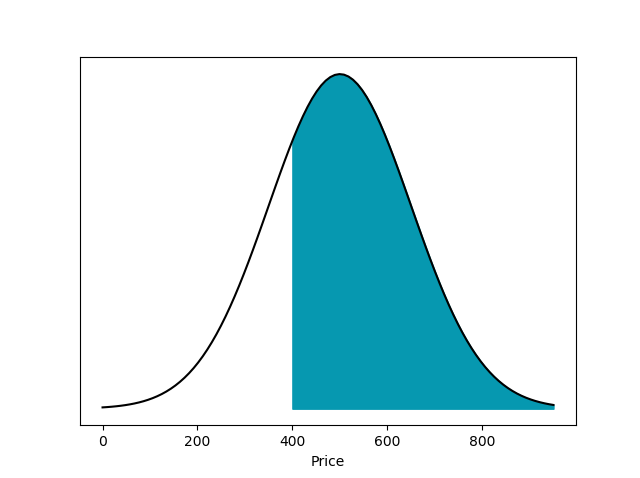
\includegraphics[width=\linewidth]{ND_integral}
						\caption{ВП}\label{Fig:Data1}
					\end{minipage}$\longrightarrow$
					\begin{minipage}{0.48\textwidth}
						\centering
						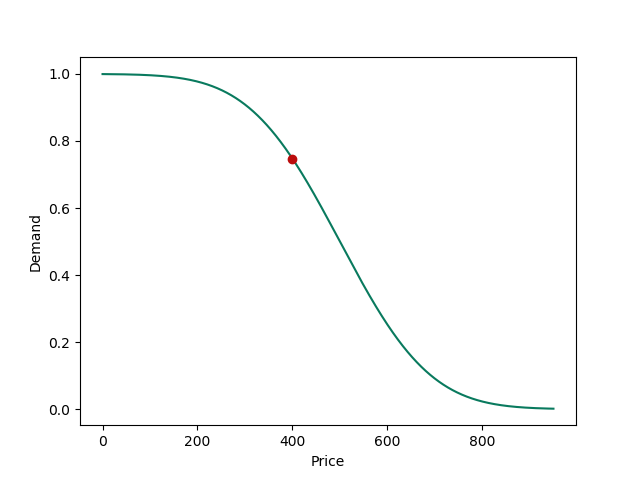
\includegraphics[width=\linewidth]{Sample_point}
						\caption{Цена и търсене}\label{Fig:Data2}
					\end{minipage}
				\end{figure}\par\noindent
				Отбелязаме, че интегралът трябва да бъде изчилсен до безкрайност, но след като $k$ стигне $\mu+3\sigma$, резултатът става пренебрежимо малък. Правейки това за цялата функция на разпределението получаваме кривата на търсенето чрез процента хора, които биха платили. Нека означим кривата на търсенето с $F(x)$:
				$$
				F(x)=
				\begin{cases}
					\dfrac{1}{2}\left (1-\operatorname{erf}\left (\dfrac{z}{\sqrt{2}}\right )\right ) 	\text{ако } x>\mu,\\
					\\
					\dfrac{1}{2}\left (1+\operatorname{erf}\left (\dfrac{z}{\sqrt{2}}\right )\right ) \text{ако } x<\mu.
				\end{cases}
				$$\par
				Искаме да оптимизираме броя хора във всяка тестова група. Математическата функция, която искаме да опишем ни дава възможността да изчислим грешките от експерименталните данни с максимална точност.
				\begin{figure}[H]
					\begin{minipage}{0.48\textwidth}
						\centering
						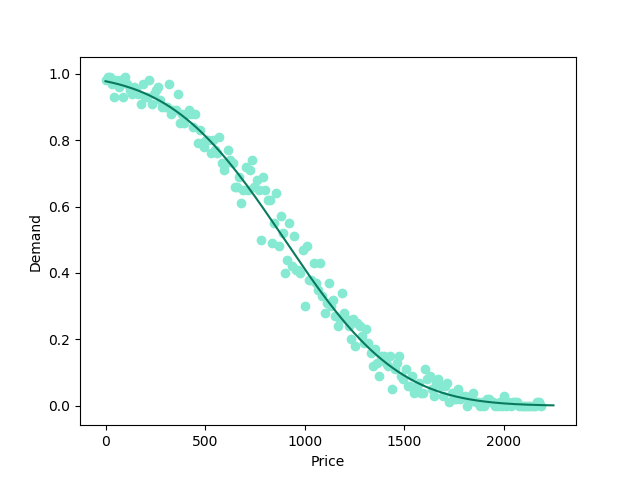
\includegraphics[width=\linewidth]{Exp_and_math_100}
						\caption{100 човека в групата}\label{Fig:Data3}
					\end{minipage}\hfill
					\begin{minipage}{0.48\textwidth}
						\centering
						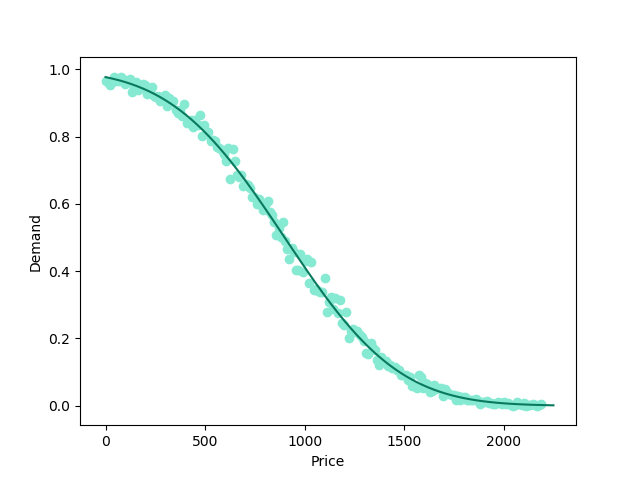
\includegraphics[width=\linewidth]{Exp_and_math_400}
						\caption{400 човека в групата}\label{Fig:Data4}
					\end{minipage}
				\end{figure}\par\noindent
				Събирайки информация за размера на тестовата груап и грешките, съставяме графика, която показва тези промени.
				\begin{figure}[H]
				\begin{minipage}{1.0\textwidth}
					\centering
					\includegraphics[width=0.7\textwidth]{\dq Error vs sample size 4\dq}
					\caption{Тестов размер и грешка}\label{Fig:Data5}
				\end{minipage}
				\end{figure}
			%\subsubsection{Архивираща функция}
			%	В тази секция описваме функция, отговаряща за вероятността за присъствието на архив. Изчислен е ефектът и върху очакваната печалба.\par
			%	Първо нека дефинираме архивния итератора $b$: 
			%	$$
			%	b=
			%	\begin{cases}
			%		1 \text{ ако жертвата има архив},\\
			%		0 \text{ ако жертвата няма архив}
			%	\end{cases}
			%	$$
			%	Сега нека дефинираме желанието за плащане (ЖЗП):
			%	$$
			%	P(x)=
			%	\begin{cases}
			%	d_{x} \text{ ако } b_{i}=0,\\
			%	c \text{ ако } b_{i}=1
			%	\end{cases}
			%	$$
			%	Тук цената на архив е означена с $c$, а цената на данните на жертвата- с $d_{x}$.\par
			%	Както и по-рано, изчисляваме очакваната вероятност даден човек да плати цена $x$.
			%	Приемаме, че вероятността конкретна жертва да има архив е константа $p$ и изследваме как промяната на тази стойност влияе на очакваната печалба. Чрез събраните данни създаваме графика, която показва връзката между двете променливи. Измерената грешка е относителна.
			%	\begin{center}
			%		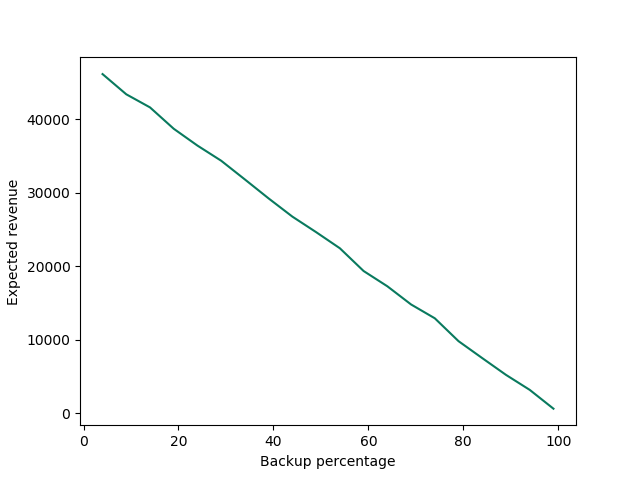
\includegraphics[width=0.55\textwidth]{Revenue_vs_backup}
			%	\end{center}		
		\subsection{Резултати}
			Изследвахме как размерът на тестовата група влияе на грешката на експерименталните данни и също как процента на защитените с архиви влияе на очакваната печалба. Моделът се фокусира на оптимизирането на цената на откупа, но авторът вярва, че за да можем да предприемем подходящи предпазни мерки срещу атаки от този вид, трябва да разбираме всеки ход на престъпниците. Поставяйки се на мястото на извършителите е ключово за целта. Допълнителни резултати, като връзката между очакваната печалба и броя на хората с архиви може да ни помогне да стигнем до подходящи подходи за справяне със заплахата.
	\section{Оптимизиране на архивирането}
		\subsection{Въведение}
			Когато става дума за защита от рансъмуер, най-ефективният метод са архивите. Те на свой ред трябва да бъдат създавани регулярно, защото ефектът от тях при потенциална атака иначе би бил незначителен. Затова е важно протоколите за архивиране да са съставени внимателно и да са съобразени едновременно с рисковете от атака и с нужните за тях ресурси. Нещо повече, оптимизирането на бекъпи може едновременно да увеличи сигурността и да намали разходите.\par
			В тази част на проекта е разгледан модел на архивиране с цел да бъде изчилсена очакваната цена. Подобни модели, разглеждащи пълйни и инкрементални архиви, са създавани и изследвани и преди\cite{nakamura2003optimal}\cite{qian2010optimal}. Разглеждаме цикъл от архиви, който се повтаря между два пълни архива и изследваме как интервалите влияят на очакваната цена на възстановяване и колко бързо ефектът, породен от първоначално незащитените данни преди първия пълен архив, намалява с времето.
		\subsection{Теоретична постановка}
			Настоящият модел е създаден с идеята да изчисли и оптимизира очакваната цена на възстановяване в случай на атака.\par
			Ще разглеждаме ахивът като структура от данни със следните качества:
			$$
			B
			\begin{cases}
			d \text{: the date on which the backup was made, as a day difference from a starting point}\\
			p \text{: the probability that the recovery is unsuccessful for any reason}\\
			r \text{: the price of trying to recover the data from the given backup}
			\end{cases}
			$$
			Два вида архиви са разгледани:
			\begin{enumerate}
				\item Full backup: a backup of the whole database
				\item Incremental backup: only saves the changes from the last backup
			\end{enumerate}
			Атхивите от конкретен вид имат обща вероятност за провал и цена за опит за възстановяване. \par
			За да може един инкрементален архив да е успешен, трябва всички инкрементални архиви преди него до успешен пълен архив също да са успешни, както и самият пълен архив.\par
			В случая цената на данните трябва да се разглежда от субективна гледна точка. Дори и на пазара данните да нямат голяма стойност, ако те са фундаментални за функционирането на компанията, тя ще е готова да плати много за незабавното им възстановяване. Следователно, в описания модел цената на данните се разглежда като вечно увеличаваща се величина и с целите на изследването "скоростта на работа", именно цената на данните, генерирани за един ден, на компанията се счита за константа. Ще я означим с $w$.\par
			Цената на възстановяването на архив ще се разглежда като сума от два фактора:
			\begin{itemize}
				\item Цената на изработването на загубените данни, означена с $W$
				\item Цената на процеса по възстановяването, означена с $R$
			\end{itemize}.
			Дефинираме $W = \Delta t.w$, където с $\Delta t$ означаваме разликата в дни между датана на успешно възстановения архив и датата на атаката, и $R = \sum_{i=1}^{n} r_i$, където броят опити за възстановяване $n$ и 
			$$
			S=\Delta t.w + R,
			$$
			Нека разликата в дни между първият архив и датата на атаката е $T$. В случай, че никой от пълните архиви не се окаже успешен, въвеждаме променлива $W_T$, съответстваща на цената на преработване на цялата работа от начало. Ясно е, че $W_T>T.w$\par
		\subsection{Само пълни архиви}
			Когато разглеждаме само пълни архиви, моделът е разпределение на Бернули с краен брой опити, а именно броят пълни архиви. Спираме, когато успеем да намерим успешен архив, започвайки от последния и вървейки към първия. Да дефинираме свойствата на пълен архив($B_F$):
			$$
			B_F
			\begin{cases}
			p_F: \text{вероятността за провал}\\
			r_F: \text{цената за опит за възстановяване}\\
			t_F: \text{дните между два последователни пълни архива}\\
			\end{cases}
			$$
			Нека $k$ е броят пълни архиви направени преди деня на атаката. Тогава:
			$$
			k = \left \lfloor{\frac{T}{t_F}}\right \rfloor + 1
			$$
			Сега можем да дефинираме очакваната цена на възстановяване:
			\begin{equation}
			\label{eq:1}
			E(T) = p_F^{k}\left(W_T + k.r_F\right) + \displaystyle \sum_{i=0}^{k-1} (1-p_F).p_F^{i}\left( \left (\left\{ \frac{T}{t_F}\right \} + i\right)t_F.w + (i+1).r_F \right )
			\end{equation}
			Направените изчисления са ключови поради невъзможността инкременталните архиви да бъдат възстановени без работещ пълен архив и следователно намирането на такъв е първият ни приоритет. Сега можем да разгледаме инкременталните архиви при работещ пълен архив.
		\subsection{Инкрементални архиви с работещ пълен архив}
			Ще разгледаме случая, когато имаме работещ пълен архив и се опитваме да възстановив допълнителни данни чрез инкрементални архиви.\\
			\begin{tikzpicture}
			[every node/.style={inner sep=0pt}]
			\node (1) [circle, minimum size=50.0pt, fill=teal, line width=0.625pt, draw=black] at (50.0pt, -130pt)  {};
			\node (2) [circle, minimum size=31.25pt, fill=lime, line width=0.625pt, draw=black] at (135pt, -130pt)  {};
			\node (3) [circle, minimum size=31.25pt, fill=lime, line width=0.625pt, draw=black] at (220pt, -130pt)  {};
			\node (4) [circle, minimum size=31.25pt, fill=lime, line width=0.625pt, draw=black] at (305pt, -130pt)  {};
			\node (5) [circle, minimum size=50.0pt, fill=teal, line width=0.625pt, draw=black] at (390pt, -130pt)  {};
			\draw [line width=0.625, ->, >=latex, color=black] (1) to  (2);
			\draw [line width=0.625, ->, >=latex, color=black] (2) to  (3);
			\draw [line width=0.625, ->, >=latex, color=black] (3) to  (4);
			\draw [line width=0.625, ->, >=latex, color=black] (4) to  (5);
			\end{tikzpicture}\\
			Нека дефинираме свойствата на инкременталните архиви ($B_I$) по подобен начин:
			$$
			B_I
			\begin{cases}
				p_I: \text{вероятността за провал}\\
				r_I: \text{цената за опит за възстановяване}\\
				t_I: \text{дните между два последователни инкрементални архива}\\
			\end{cases}
			$$
	\newpage
			Нека с $T_F$ да означим разликата в дни между денят на атаката и датата на успешния пълен архив и с $l$ да означим броят инкрементални архиви, които трябва да разгледаме. Имаме две опции за $l$ в зависимост от това дали последният пълен архив е бил успешно възстановен:
			$$
			l=
			\begin{cases}
			\left\lfloor \frac{T_F}{t_I}\right \rfloor \text{, ако } T_F<t_F\\
			\left\lfloor \frac{t_F}{t_I}\right \rfloor -1 \text{, ако } T_F>t_F\footnotemark\\
			\end{cases}
			$$
			\footnotetext{Можем да опитваме да възстановим само инкрементални архиви предхождащи следващият пълен архив}
			Да отбележим, че това последният пълен архив да е успешен е еквивалентно на $T_F<t_F$.\par
			Сега сме в точно обратната ситуация спрямо миналата част. Процесът по възстановяване на инкрементални архиви продължава докато не се натъкнем на провал, тъй като това би означавало, че всички следващи инкрементални архиви също са неизползваеми. С това намаляме $W$, тъй като в началната позиция сме готови да преработим данните до датата на успешния пълен архив. Сега сме готови да изчислим очакваната цена:
			\begin{equation}
				\label{eq:2}
				f(T_F) = (1-p_I)^l.((T_F-t_I.l).w + r_I.l) + \displaystyle \sum_{i=0}^{l-1} (1-p_I)^{i}.p_I((T_F-t_I.i)w + r_I.(i+1))
			\end{equation}
			Сега знаем колко ще намалее цената на възстановяването, когато използваме инкрементални архиви, и можем да построим цялостния модел, използвайки уравнения \ref{eq:1} и \ref{eq:2}.
		\subsection{Крайна очаквана цена}
			Към всяко събираемо в уравнение \ref{eq:1} Трябва да добавим ефектът на инкременталните архиви и получаваме нови събираеми от вида:
			$$
			P(W + R),
			$$
			където $P$ е вероятността определена комбинация от събития да се случи, $W$ е цената на данните, които трябва да бъдат създадени наново, а $R$ е цената на процесът по възстановяването. Инкременталните архиви намаляват цената на данните, които трябва да бъдат създадени наново, но увеличават $R$. Както споменахме по-горе, има само един случай, вкойто броят инкрементални архиви, които трябва да имаме предвид е различен и той е именно този, в който последният пълен архив е възстановен успешно. Ако $i$-тият пълен архив е успешен\footnote{Това съответства на $i-1$-вото събираемо в сумата от уравнение \ref{eq:3}}:
			$$
			T_F=t_F\left(\left\{ \frac{T}{t_F} \right\} + i - 1\right)
			$$
			Комбинирайки уравнения \ref{eq:1} и \ref{eq:2} получаваме:
			\begin{equation}\label{eq:3}
			F(T) = p_F^{k}(W_T+k.r_F) + \displaystyle\sum_{i=0}^{k-1}(1-p_F).p_F^{i}\left(f(T_F) + (i+1).r_F\right)
			\end{equation}
			Използвайки уравнения \ref{eq:1} и \ref{eq:3}, можем да построим графика на очакваната цена с и без използването на инкрементални архиви.
			\begin{figure}[H]
				\begin{minipage}{1.0\textwidth}
					\centering
					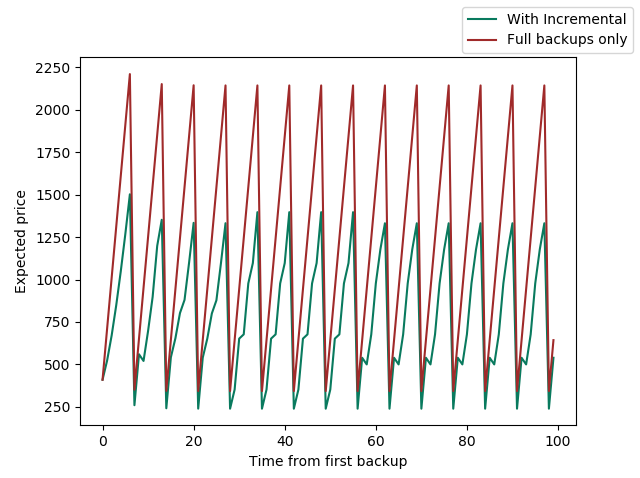
\includegraphics[width=0.7\textwidth]{Weekly_full.png}
					\caption{Full only and Whole model}\label{Fig:FullWeekly}
				\end{minipage}
			\end{figure}
		\subsection{Симулация Монте Карло}
			Направена бе симулация от тип Монте Карло на python, която генерира случайни процеси на възстановяване на данни с описаната структура на архивите. Цената на възстановяването беше направена на графика спрямо датата на атаката:
			\begin{figure}[H]
				\begin{minipage}{1.0\textwidth}
					\centering
					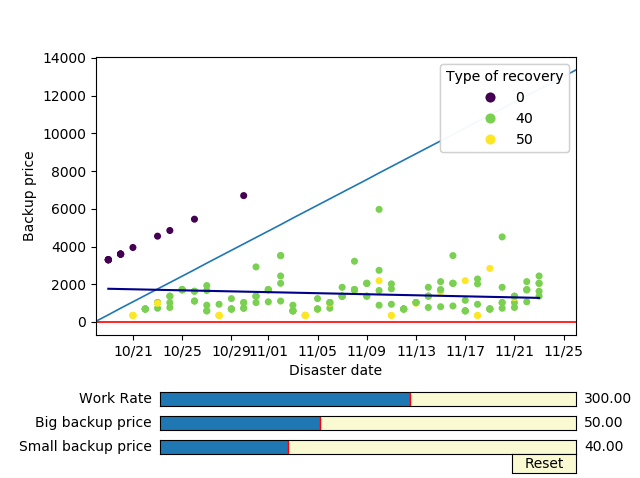
\includegraphics[width=0.7\textwidth]{Weekly_full_carlo.png}
					\caption{Симулация Монте Карло}\label{Fig:MonteCarlo}
				\end{minipage}
			\end{figure}
			\blfootnote{Във фигура \ref{Fig:FullWeekly} и фигура \ref{Fig:MonteCarlo} данните са за седмичен пълен архив и ежедневен инкрементален}
			Цветовете във фигура \ref{Fig:MonteCarlo} показват вида на последния успешно възстановен архив, пълен, инкрементален или несъществуващ.
			\newpage
			Линейна регресия на данните беше генерирана, която показва ефектът от начално неподсигурените данни изчезва с времето, тъй като цената при провал се изчилсява като цената за преработването на всички данни, които компанията е генерирала.
		\subsection{Резултати}
			Беше построен модел за изчисляване на очакваната цена при възстановяване на данни. Нещо повече, ефектът от инкременталните архиви беше показан в сравнение със стратегия използваща само пълни архиви. Беше направена и анализирана симулация от тип Монте Карло, коятодемонстрира реалния процес на възстановяване.
	\section{Бъдещо развитие}
		Авторът разглежда няколко посоки за бъдещото развитие на проакта, а именно:
		\begin{itemize}
			\item разглеждане на неконстантна скорост на работа за модела за архивиране
			\item разширяване на модела за откуп в посока описване на по сложни начини за разпространение на рансъмуера.
			\item използване на резултатите и базите данни на подобни проучвания с цел подкрепянето на модела с реални данни.\cite{paquet2019ransomware}
			\item използване на динамичен модел за оценка на откупа
		\end{itemize}
	\section{Благодарности}
		Искам да благодаря на своя ментор, Явор Папазов, и на Константин Делчев за безотказната помощ в избора на темата на проекта и последващото му развитие, за снабдяването ми с всички нужни материали за запознаването ми с темата, както и за изслушването на въпросите ми. Искам също да благодаря на Станислав Харизанов за професионалните съвети.
\nocite{*}
\bibliographystyle{unsrt}
\bibliography{Bibliography}
\end{document}